\chapter{Objetivos}\label{cap.objetivos}
Una vez introducido el contexto en que se ha desarrollado este trabajo, es hora de profundizar en los objetivos concretos que se han tratado de alcanzar, los requisitos para las soluciones desarrolladas y la metodología que se ha seguido para conseguirlos.

\section{Objetivos}
La meta planteada en este proyecto es la mejora de la plataforma educativa \textit{Robotics-Academy} utilizando el \textit{software} robótico ROS y el entorno web \textit{Jupyter}, además de la creación de una práctica completamente nueva, llamada \textit{Chrono}, y la actualización de una de las prácticas existentes en esta plataforma, llamada \textit{Follow Road}, así como una actualización de sus \textit{drivers} para que soporte \textit{ROS} y su inclusión en la infraestructura web de Robotics-Academy-Web.

La primera práctica consiste en la competición de dos coches de F1 por un circuito que dispone de una línea roja que se debe seguir. El código del alumno competirá con el F1 del mejor tiempo registrado, de menor tiempo posible, para el circuito en el que esté compitiendo. De esta manera conseguiremos que el alumno pueda depurar su código de solución y tenga un estímulo para alcanzar la perfección en el desarrollo de su algoritmo.

En cuanto a la segunda práctica, trata de un dron con una cámara que debe seguir una carretera. El código del alumno deberá filtrar las imágenes para segmentar la carretera y dotar de un movimiento controlado al dron que le permita seguir la carretera. Esta práctica ha sido actualizada para que funcione con la nueva infraestructura \textit{software} de los drones (\textit{ROS} y \textit{MavROS}, además de realizar una versión del ejercicio con cuadernillo de \textit{Jupyter}.

\section{Requisitos}
Además de lograr los objetivos, los requisitos necesarios que se van a exigir al software desarrollado son:

\begin{enumerate}
	\item El Sistema Operativo empleado será Ubuntu 16.04 LTS.
	\item Se utilizará el \textit{middleware} robótico JdeRobot en su versión 5.6.2. El uso de este \textit{middleware} robótico simplifica la programación de comportamientos en los robots.
	\item Se usará \textit{OpenCV3} para el procesamiento de las imágenes captadas por las cámaras en ambas prácticas.
	\item Para dar soporte a los sensores y actuadores se utilizará \textit{ROS-Kinetic}, que es el estándar de facto en la comunidad robótica.
	\item Para mostrar el comportamiento de los robots se utilizará el simulador \textit{Gazebo}, uno de los más completos y utilizados en la actualidad.
	\item El lenguaje de programación utilizado para el desarrollo de ambas prácticas será \textit{Python} en su versión 2.7.12, por compatibilidad con el \textit{middleware} robótico \textit{ROS-Kinetic}.
	\item Las soluciones desarrolladas deben ejecutar algoritmos en tiempo real, por lo que deben ser eficientes y realizar movimientos suaves.
\end{enumerate}

\section{Metodología}
El desarrollo de este Trabajo de Fin de Grado puede descomponerse en un conjunto de iteraciones con distintas fases. Cada fase está formada por una reunión semanal con el tutor para determinar los objetivos a abordar, la planificación de cómo abordarlos, intentar solucionar los problemas que vayan a surgir anticipadamente y la consecución de los objetivos durante la semana. De esta manera se ha conseguido un desarrollo fluido y completo, asentando los conocimientos y despejando las dudas que surgían durante los meses dedicados a este desarrollo.

Además de las reuniones semanales, se han utilizado herramientas de apoyo como la bitácora semanal en la Wiki de JdeRobot\footnote{\url{https://jderobot.org/Pablomoreno-tfg}}, donde se redactaban los avances obtenidos acompañados de vídeos demostrativos e imágenes. Además, el código creado se desarrollaba, progresivamente, en la plataforma Github, en un repositorio personal\footnote{\url{https://github.com/RoboticsURJC-students/2017-tfg-pablo-moreno}} \footnote{\url{https://github.com/PabloMorenoVera/Academy}}, a los cuales el tutor tiene acceso para dar realimentación y orientar el proceso.

 El modelo de desarrollo escogido ha sido el modelo creado por Barry Boehm. Al tratarse de un modelo en espiral, se adaptada a la perfección a nuestras necesidades, permitiendo disponer de flexibilidad ante cambios en los requisitos semanales, algo común mientras avanzaba el desarrollo. En paralelo, nos permitía separar el objetivo final en varias sub-tareas más sencillas. Con esto se ha conseguido una subsanación de los riesgos temprana y la definición de una arquitectura en las fases iniciales del desarrollo, todo ello dotado con un control de calidad continuo.

\begin{figure}[H]
  \begin{center}
    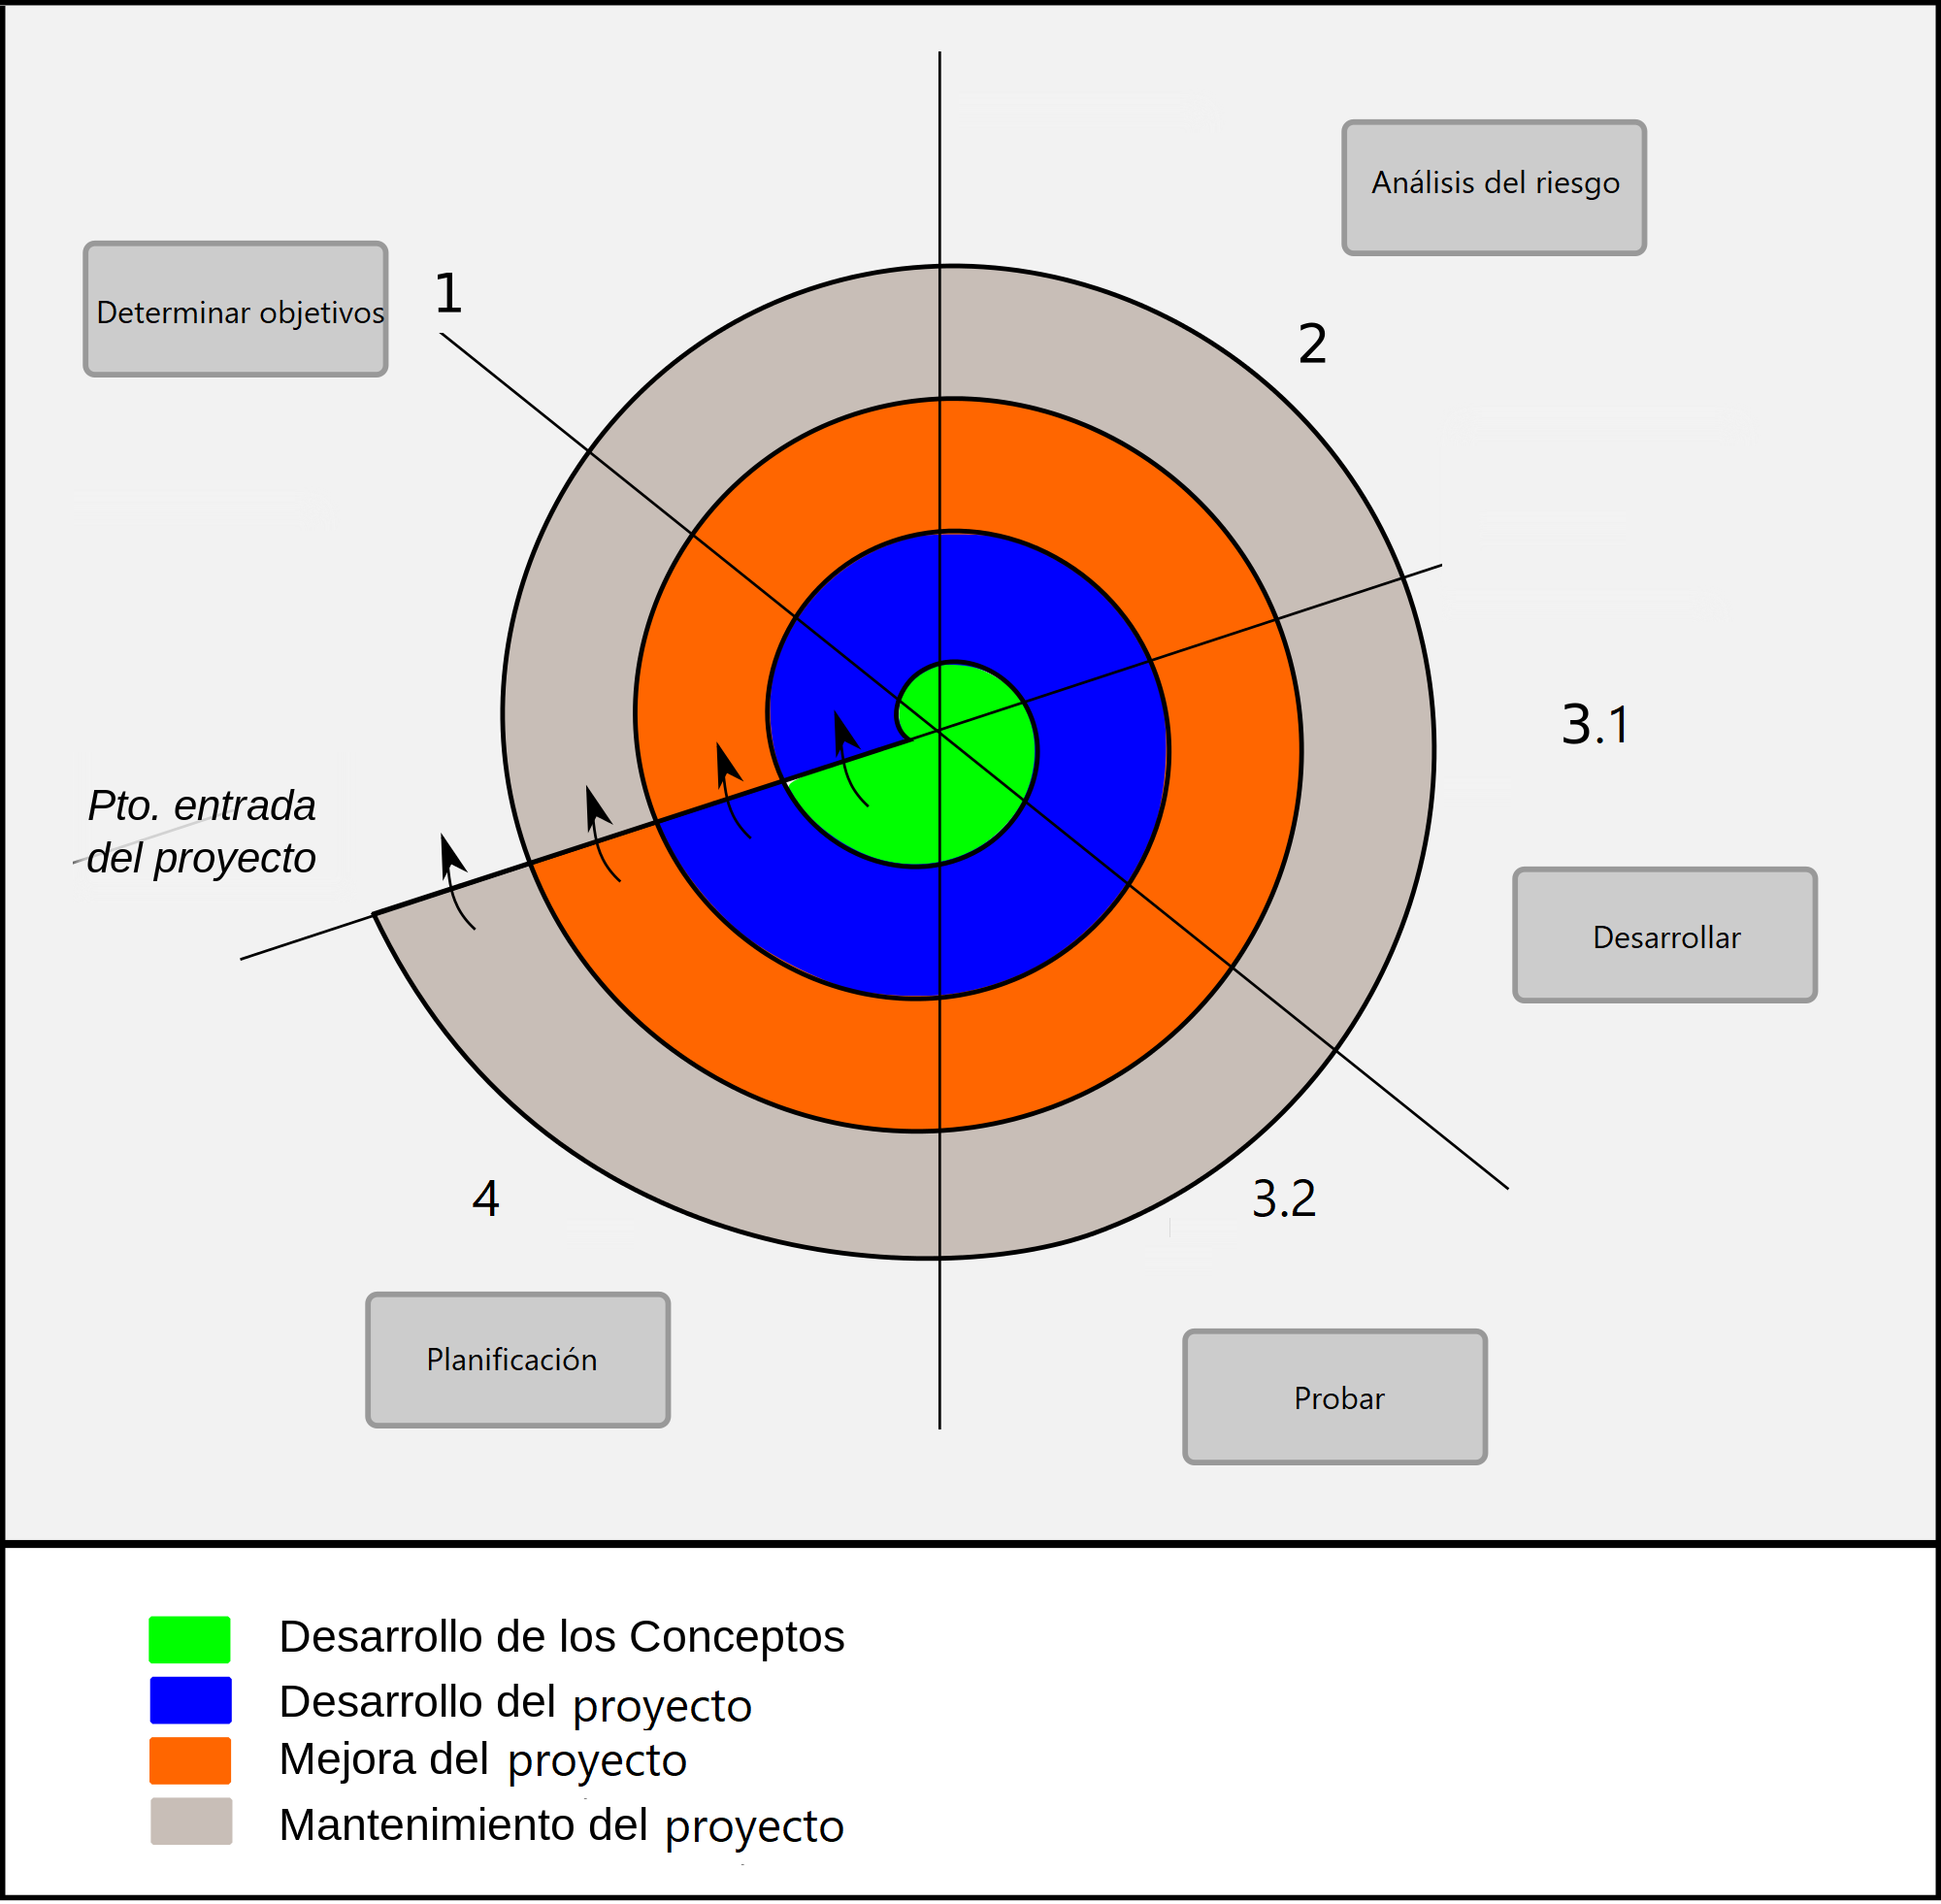
\includegraphics[width=0.55\linewidth]{figures/modelo_espiral.png}
		\caption{Modelo de desarrollo en espiral}
		\label{fig.espiral}
		\end{center}
\end{figure}

La ventaja de este ciclo de vida es que permite la obtención de prototipos funcionales en una etapa temprana, la optimización progresiva del prototipo desarrollado y, en última instancia, pulir los detalles para abarcar la totalidad de los requisitos especificados (Figura 2.1). De esta manera el trabajo se desarrolla de manera incremental con cuatro fases bien definidas:

\begin{itemize}
	\item[--] \textbf{Determinar objetivos}: Esta primera fase del ciclo está formada por la definición de las metas.
	\item[--] \textbf{Análisis del riesgo}: Se evalúan los posibles problemas iniciales al desarrollo y las soluciones a los mismos.
	\item[--] \textbf{Desarrollar y probar}: En esta tercera fase se procede al desarrollo del trabajo propiamente dicho, junto con una serie de pruebas para verificar su funcionamiento.
	\item[--] \textbf{Planificación}: En esta última fase del ciclo se valoran los resultados obtenidos y se planifican las siguientes etapas del proyecto.
\end{itemize}

\section{Plan de trabajo}
Para la consecución de los objetivos descritos, se han seguido seis etapas de trabajo:

\begin{itemize}
	\item[--] \textbf{Estudio de JdeRobot y el entorno educativo \textit{Robotics-Academy}}: una vez descargado e instalado tanto el software, dependencias y bibliotecas como el simulador, se tomará un primer contacto con el entorno JdeRobot mediante la modificación y readaptación de algunas prácticas existentes, como sus interfaces gráficas.
	\item[--] \textbf{Estudio de \textit{ROS-Kinetic} y del simulador Gazebo}: esa etapa se ha dedicado al desarrollo de algunos modelos en el simulador, estudiando ejemplos disponibles en la web\footnote{\url{http://gazebosim.org/tutorials}} y en JdeRobot, así como modificándolos y desarrollando algunos modelos nuevos. En esta etapa también se han estudiado el funcionamiento básico de los \textit{plugins} que dispone Gazebo para el control de sus robots, sensores y actuadores. Esto ha supuesto una toma de contacto con el lenguaje de programación C++ utilizado, también, para comprender los \textit{plugins} de ROS-Kinetic.
	\item[--] \textbf{Actualización de la infraestructura del dron sigue-carretera}: Esta práctica estaba bastante obsoleta y se procedió a renovar por completo su interfaz gráfica, el escenario utilizado incluyendo un nuevo dron que soportaba ROS y una nueva conexión de los sensores y actuadores del propio dron. Se desarrolló una optimización global del nodo académico como la inclusión de una pausa académica. Además, se creó una versión de la práctica para la plataforma Jupyter y se incluyó en el elenco de prácticas soportadas en \textit{Robotics-Academy}.
	\item[--] \textbf{Desarrollo de una solución de referencia para la práctica dron sigue-carretera}: Mediante la utilización de filtros de color y control PID.
	\item[--] \textbf{Desarrollo de la infraestructura del ejercicio F1-chrono}: Se desarrolló el modelo del F1 y el circuito para competir en \textit{Blender} y \textit{SketchUp} para conformar el escenario de Gazebo. Se utilizaron los drivers del robot F1 ya existentes para dar soporte en ROS-Kinetic de los motores. la cámara y el láser. Se creó el nodo ROS de la práctica para alojar el código del estudiante y la versión de la práctica para Jupyter.
	\item[--] \textbf{Desarrollo de una solución de referencia para F1-chrono}: Con algoritmos de filtros de color y control PID.
\end{itemize}